In Kapitel \ref{chp:interaktion_mit_multitoucheingaben} wurden einige bekannte Ansätze zur Interaktion durch Multi-Touch Eingaben vorgestellt. Diese werden im Rahmen dieser Arbeit als explizite 3D Multi-Touch Techniken bezeichnet. Wir definieren explizite Multi-Touch Navigation als Strategie, mit welcher verschiedene Freiheitsgrade der Manipulation durch Nutzereingaben direkt steuerbar sind.
\\\\
In diesem Kapitel wird beschrieben wie anhand dieser Techniken Gesten für die, im Rahmen dieser  Arbeit entstandene Applikation zur touch- basierten Navigation, abgeleitet wurden. Abschnitt \ref{sec:rst_im_bildraum} erläutert die Integration der Rotation, Translation und Skalierung im Bildraum, welche im Folgenden mit RTS abgekürzt wird. Abschnitt \ref{sec:3d_translation} zeigt wie alle Freiheitsgrade der dreidimensionalen Translation in einer Navigationsgeste bedient werden können. In Abschnitt \ref{sec:3d_rotation} wird ein Ansatz zur Steuerung aller Freiheitsgrade der dreidimensionalen Rotation vorgestellt. Abschließend werden in Abschnitt \ref{sec:vorteile_und_limitierungen_explizit} die vorgestellten Techniken gegenübergestellt und auf ihre Vorteile und Limitierungen untersucht.


\section{Rotation, Translation und Skalierung im Bildraum}
\label{sec:rst_im_bildraum}

Zur Umsetzung der RTS-Technik dienen die Erkenntnisse von CITE STICKYTOOLS. Nach dieser Strategie soll zu jedem Zeitpunkt der Interaktion eine orthogonale Verbindung, zwischen der Eingabeposition auf dem Bildschirm und der darunter liegenden Geometrie, bestehen.
\\\\
Wird zur Berechnung der Manipulation ein Kontaktpunkt auf dem Bildschirm verfolgt, können mit diesem Ansatz x- und y-Translation der Navigation gesteuert werden. Hierzu ergibt sich die Verschiebung des Viewing-Setups, aus der relativen Bewegung des Kontaktpunkts auf der Projektionsfläche. 
\\\\
Wir definieren $P_1(t) = (x_1, y_1)$ als die Position des Kontaktpunkts $P_1$ auf der Bildebene, zu einer gegebenen Zeit $t$. $P_1(t‘) = (x_1‘, y_1‘)$ sei die Position von $P_1$ zu einer späteren Zeit $t‘$. Die relative Translation $T_r = (x_r, y_r)$ berechnet sich durch $T_r = P_1(t) – P_1(t‘)$. Um diese Bewegung auszugleichen muss die Navigation um $T = (x_t, y_t) = (-x_r, -y_r)$ verschoben werden. Abbildung XX veranschaulicht diesen Zusammenhang.
\\\\
Mit der Verwendung eines zweiten Kontaktpunkts $P_2$ auf dem Bildschirm, wird diese Transformation um die Rotation entlang der Bildschirmnormalen, sowie die symmetrische Skalierung erweitert. Als Referenzpunkt hierfür dient $P_1$.
\\\\
Sei $P_2(t) = (x_2, y_2)$ die Position des Kontaktpunkts $P_2$ auf der Bildebene, zu einer gegebenen Zeit $t$ und $P_2(t‘) = (x_2‘, y_2‘)$ die Position von $P_1$ zu einer späteren Zeit $t‘$, so ergibt sich $V = P_2(t) – P_1(t)$, als Richtungsvektor zwischen den Kontaktpunkten vor der Bewegung. $V‘ = P_2(t‘) – P_1(t‘)$ ist folglich der Richtungsvektor nach der Bewegung. Verändert sich die Distanz der Kontaktpunkte auf der Tischfläche, so muss sich die Distanz der Angriffspunkte auf der Geometrie in gleichem Maße ändern. Abbildung XX zeigt wie die Skalierung der Projektionsfläche einer virtuellen Kamera, die Größenrelation der dargestellten Geometrie beeinflusst. Der Skalierungsfaktor $S$, bestimmt sich nach diesem Zusammenhang aus dem Verhältnis der Distanzen zwischen den Kontaktpunkten zu den Zeiten $t$ und $t‘$. Folglich gilt $S = |V| / |V‘|$. 
\\\\
Für die Rotation dienen ebenfalls die Vektoren $V$ und $V‘$ zur Berechnung. Als Achse dient die Bildschirmnormale $N$. Diese kann leicht durch $N = ||V|| \times ||V‘||$ bestimmt werden. Der Winkel $\alpha$ für die Transformation ist durch $\alpha = arccos(||V|| * ||V‘||)$ gegeben.


\section{3D Translation}
\label{sec:3d_translation}

Die 3D Translation ist einer von den Erkenntnissen der Balloon Selection nach Benko und Feiner \cite{benko:2007} abgeleiteter Ansatz. Durch Berühren  der Tischfläche mit einer Hand wird eine direkte Verbindung mit der darunter liegenden Geometrie hergestellt. Diese zur Tischfläche orthogonale Beziehung soll zu jedem Zeitpunkt der Navigation in diesem Modus gewahrt bleiben. Es leitet sich demnach für die Interaktion mit nur einem Eingabepunkt eine zweidimensionale Translation, nach den in Abschnitt \ref{sec:rst_im_bildraum} beschriebenen Zusammenhängen, ab.
\\\\
Durch die Verfolgung der Bewegung zweier Eingabepositionen, kann eine dreidimensionale Translation abgebildet werden. Hierzu dient einer der verfolgten Kontakte auf dem Tisch, als Primäreingabe. Die Bewegung dieser Position bestimmt weiterhin die x- und y-Translation im Bildraum. Der zweite Kontakt wird im Folgenden als Sekundäreingabe bezeichnet. Die Einordnung in Primär- und Sekundäreingabe kann durch Auswertung der Startzeit der jeweiligen Eingabe festgelegt werden. Durch Distanzveränderung der Sekundäreingabe zur Primäreingabe kann die z-Verschiebung gesteuert werden. Zur Berechnung dieser bieten sich zwei verschiedene Verfahren an.
\\\\
Wir definieren $P_1(t) = (x_1, y_1)$ und $P_2(t) = (x_2, y_2)$ als die Positionen der Primäreingabe $P_1$ und der Sekundäreingabe $P_2$ auf der Projektionsfläche, zu einer gegebenen Zeit $t$. $P_1(t‘) = (x_1‘, y_1‘)$ und $P_2(t‘) = (x_2‘, y_2‘)$  seien die Position von $P_1$ und $P_2$ zu einer späteren Zeit $t‘$. Weiterhin werden die Richtungsvektoren $V = P_2(t) – P_1(t)$ und $V‘ = P_2(t‘) – P_1(t‘)$ bestimmt. $z_t$ ist die zu ermittelnde z-Translation.
\\\\
Das erste Verfahren nutzt die Differenz zwischen $|V|$ und $|V‘|$ zur Bestimmung der z-Translation. Bei Verlängerung der Distanz zwischen den Eingabepunkten, soll der Abstand zur darunter liegenden Geometrie in gleichem Maße abnehmen. Bei Verkürzung der Strecke zwischen $P_1$ und $P_2$ wächst die Distanz zur Geometrie um den Betrag der Differenz. Für ein Viewing Setup, mit Blickrichtung entlang der negativen z-Achse, ergibt sich $z_t = |V| – |V‘|$. Der entstehende Effekt lässt sich mit der Anwendung einer Seilwinde vergleichen.
\\\\
Im zweiten Verfahren wird das Verhältnis zwischen $|V|$ und $|V‘|$ zur Bestimmung der z-Translation genutzt. Verdoppelt sich beispielsweise die Strecke zwischen $P_1$ und $P_2$, so halbiert sich die Distanz zwischen $P_1$ und der Geometrie.
\\\\
TODO FORMEL FERTIG
\\\\
Abbildung \ref{fig:baloon_interaction} visualisiert den Umgang mit diesem Interaktionsmodus. Hierbei wird dem Nutzer eine Visualisierung des manipulierten Auftreffpunktes auf der Geometrie dargestellt, sowie die Verbindungslinie zur darüberliegenden Handposition. Die Gerade zwischen den Eingabepositionen wird ebenfalls visuell referenziert.

\begin{figure}
	\begin{center}
		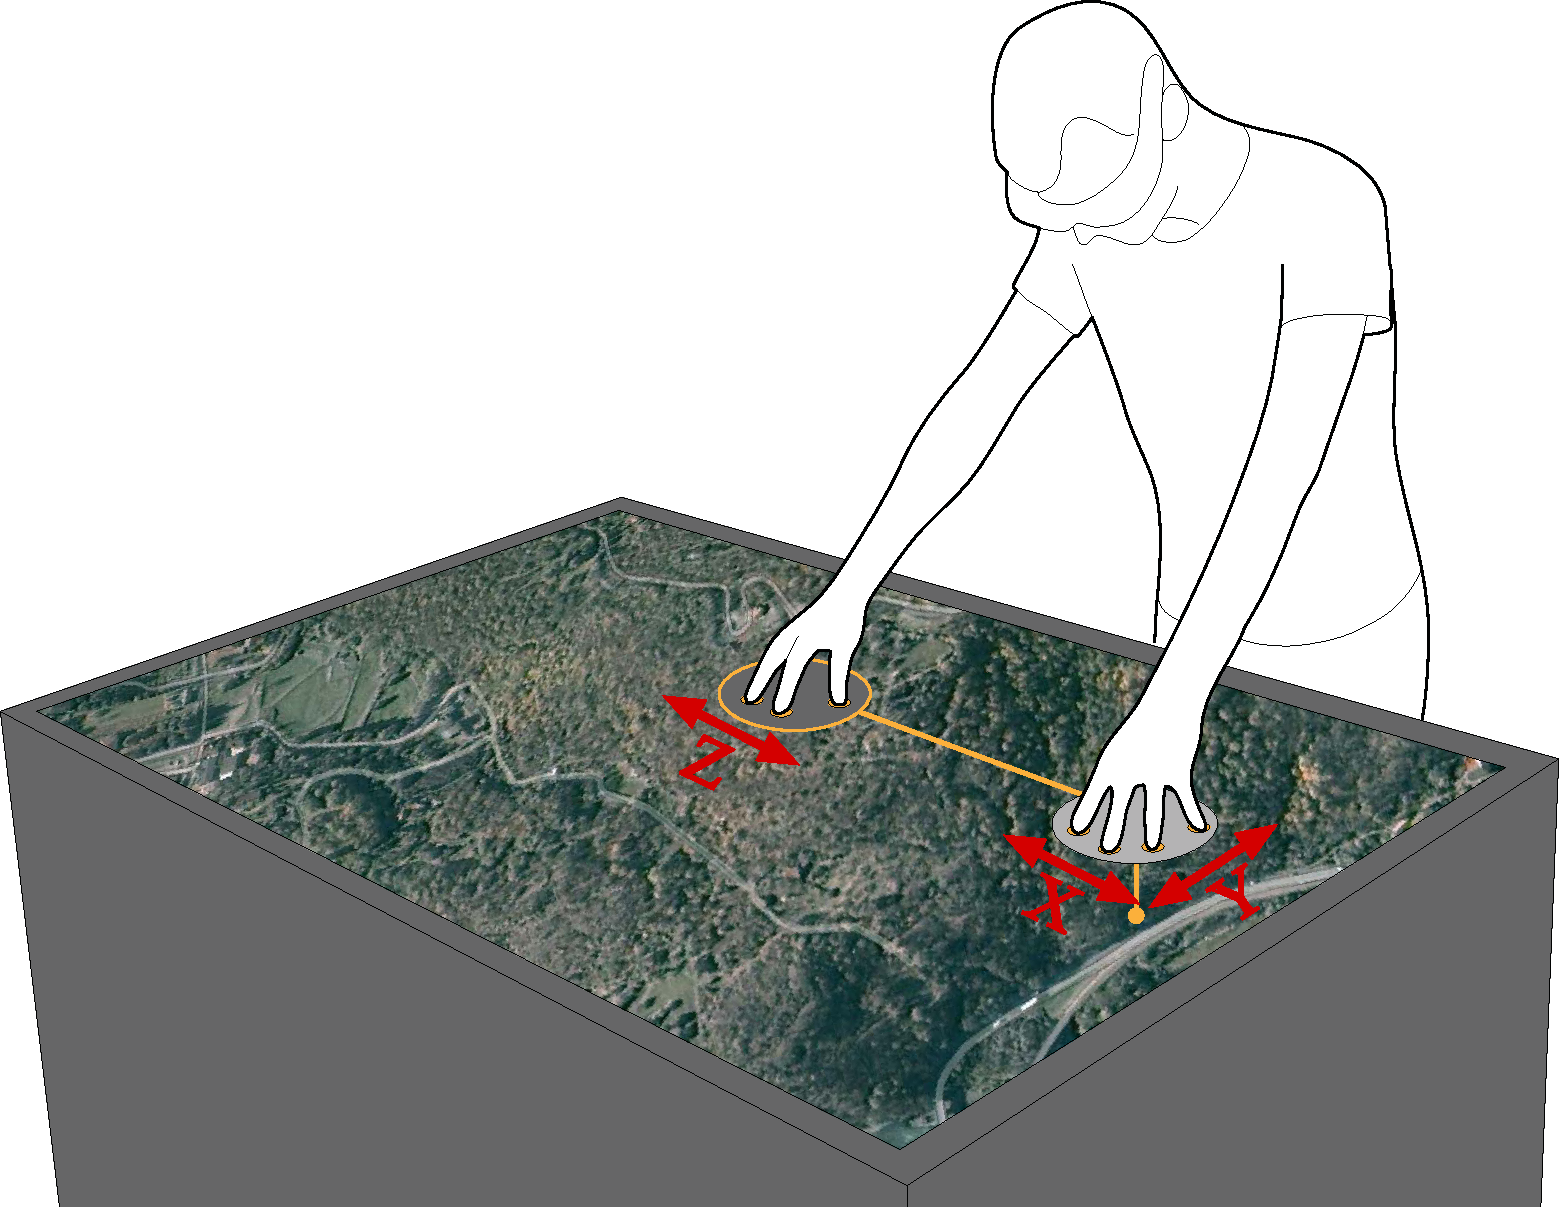
\includegraphics[width=10cm]{img/baloon_interaction.pdf}
	\end{center}
	\caption{Interaktion im 3D Translationsmodus auf Grundlage der Erkenntnisse von Benko und Feiner \cite{benko:2007}. Die roten Pfeile sowie deren Beschriftung sind nicht Teil der Interaktionsvisualisierung}
	\label{fig:baloon_interaction}
\end{figure}

\section{3D Rotation}
\label{sec:3d_rotation}

Ziel dieser Technik ist die Kontrolle aller Freiheitsgrade, welche für die Rotation im dreidimensionalen Raum benötigt werden. Hierzu wurde der in Abschnitt REF ARCBALL RELATED vorgestellte Ansatz von CITE ARCBALL implementiert. 
\\\\
Für die Bestimmung der Manipulation wird die Hand eines Nutzers mit genau zwei aufgesetzten Fingern verfolgt. Initiiert der Nutzer die Geste durch Aufsetzen der Hand, so wird ein direkter Angriffspunkt auf der Geometrie mit orthogonaler Verbindungsgeraden zur Bildschirmfläche berechnet. Bis zur Beendung der Geste, durch Anheben der Hand, erfolgt eine Rotation um diesen Punkt.
\\\\
Gegeben sind $P_h(t)$ und $P_h(t‘)$ als Positionen des Mittelpunkts der Geraden zwischen den zwei aufgesetzten Fingern zu den Zeiten $t$ und $t‘$. $P_g$ sei der beschriebene Referenzpunkt auf der Geometrie. Zuletzt sind $V_f(t)$ und $V_f(t‘)$, als zeitabhängigen Richtungsvektoren zwischen den Fingern, gegeben. Es werden für die Interaktion zwei Rotationen getrennt voneinander berechnet.
\\\\
Die Richtungsvektoren $V_{hg}(t)$ und $V_{hg}(t‘)$ ergeben sich aus der Verbindung zwischen $P_h(t)$ mit $P_g$ und $P_h(t‘)$ mit $P_g$. Die Normale auf die von den Vektoren aufgespannte Ebene bildet die Achse der ersten Rotation. Der Winkel leitet sich aus dem Winkel zwischen $V_{hg}(t)$ und $V_{hg}(t‘)$ ab. $V_{hg}(t‘)$ ist außerdem die Achse für eine zweite Rotation, deren Maß durch den Winkel zwischen $V_f(t)$ und $V_f(t‘)$ bestimmt wird. Abbildung XX stellt das Verfahren an einem Beispiel dar.


\section{Vorteile und Limitierungen}
\label{sec:vorteile_und_limitierungen_explizit}

Durch die Verwendung der RTS-Technik (siehe Abschnitt \ref{sec:rst_im_bildraum}) sind eine Vielzahl verschiedener Transformationen im dreidimensionalen Raum gleichzeitig, auch getrennt voneinander zu bedienen. Der anhaltende und direkte Kontakt mit der Geometrie vermittelt dem Nutzer das Gefühl die Szene zu greifen, was zu einer intuitiven Einarbeitung in den Umgang mit dem System führt. Die Technik ist jedoch begrenzt auf dieselben Freiheitsgrade, welche auch im zweidimensionalen Raum verwendet werden. Sie bietet daher nicht die Möglichkeit, die Navigation in jeden, durch die drei Dimensionen gegebenen, Zustand zu bewegen. Dieser Nachteil spiegelt sich bei den übrigen, in diesem Kapitel vorgestellten, Techniken noch stärker wieder. Demzufolge ist durch 3D Translation und 3D Rotation jeweils nur eine Form der Transformation steuerbar. Im Kontext ihrer Anwendung zeigen sich 3D Translation, sowie 3D Rotation, ebenfalls als nutzerfreundliche Strategien zur Manipulationen der von ihnen bestimmten Freiheitsgrade.
\\\\
Die Seilwindenstrategie bei der 3D Translation weist durch ihr direktes Mapping eine hohe Präzision und ein leicht Verständliches Interaktionskonzept auf. Durch die Maße des Tisches und die Reichweite des menschlichen Armes ist der Bewegungsrahmen für die Interaktion eingeschränkt. Ein weit entferntes Objekt in die Nähe der Projektionsebene zu bringen, erfordert somit das wiederholte Anheben und erneute Aufsetzen der Hand. Aus diesem Grund wirkt die Seilwindenstrategie, bei der Arbeit mit weit entfernten Objekten, ungeeignet. Die Translationsberechnung durch das Verhältnis von Eingabepunkt- und Geometrieabstand kann hingegen effektiv für grobe Interaktionen mit weit entfernten Objekten genutzt werden. Kleine Bewegungen auf der Tischfläche führen zu einer zunehmenden Auswirkung, je weiter das berührte Objekt vom Tisch entfernt liegt. Dementgegen ist die Auswirkung von weitreichenden Bewegungen mit Geometrieelementen in Tischebene gering. Somit entstehen leicht Missverständnisse bei der Nutzung mit bildschirmnaher Geometrie.
\\\\
Die vorgestellte 3D Rotationstechnik kann den Erhalt der Orthogonalität, zwischen dem Geometrie-Eingabe-Vektor und der Bildfläche, nicht gewährleisten. Das hebt die Metapher der direkten Berührung auf, welche sich als nutzerfreundlich erwiesen hat. Wie in Kapitel \ref{chp:wahrnehmungskonflikte_und_loesungsansaetze} beschrieben, ist 3D Multi-Touch Interaktion effektiv für Objekte in Null-Parallaxe, verwendbar. Bei der 3D Rotation können geringe Eingabeänderungen zu starken Anpassungen des Rotationswinkels führen, wenn die Distanz zwischen Eingabeposition und Rotationsreferenzpunkt gering ist. Befindet sich der Referenzpunkt auf der Tischfläche ist gar keine Berechnung der Rotation mehr möglich. Des Weiteren wird durch den Übergang zwischen Positiv- und Negativ-Parallaxe die Steuerung der Rotation invertiert.
